\documentclass[dvipdfmx,autodetect-engine]{jsreport}
\usepackage{tikz}

\usepackage{amsmath}
\usepackage{booktabs}
\usepackage{url}
\usepackage{multirow}
\usepackage[dvipdfmx]{graphicx}
\usepackage{here}

\title{隠れマルコフモデルによるヒト腸内細菌叢の状態推定}
\author{江 涵\\
学籍番号 1Y15F043–1\\
\\
早稲田大学 先進理工学部\\
電気・情報生命工学科\\ 
バイオインフォマティクス研究(指導教員 浜田 道昭)\\
\\

}

\begin{document}

\maketitle

\begin{abstract}

本研究は,隠れマルコフモデルを用いてヒト腸内細菌叢の状態推定を行うことである.ヒト腸内には様々な微生物が存在し,人の食生活やライフスタイル等の選択により日々微小な変化が起こっている.人の健康状態もヒト腸内細菌叢と関わると考えられるが,それはどのようなヒト腸内細菌叢の状態により人の健康状態に影響を及ぼすのか,解明されていない.そこで,本研究では,メタゲノム解析を行うことにより,ヒト腸内細菌叢にどのような微生物が存在しているのかを調べ,人の健康状態に影響を及ぼす状態について理解を深めようと考えている\footnote{まだ実装ができていないため、文章にはこのように書くが、実装ができてから修正するつもりである.}.

本研究では,ヒト腸内細菌叢の時系列データに対し,観測変数が多項分布に従っている隠れマルコフモデルの更新式を導入し、パラメータ推定を行う。
\end{abstract}



\setcounter{tocdepth}{2} %\listoffigures 
\tableofcontents


\chapter{序論}

\section{背景}

人の腸内には様々な細菌が存在している.この中にどのような細菌が存在するのか,また細菌叢の時間的動態は健康とどのように関連しているのかについて関心が高まっている\cite{pmid20368178}\cite{pmid21885731}.ヒト腸内細菌叢は,通常長期的に安定している\cite{pmid23828941}\cite{pmid9758810}.ホストのライフスタイルの選択によるヒト腸内細菌叢の動態が明らかになった\cite{pmid25146375}が,健康に対する潜在的な影響は観察されていない.


\section{メタゲノム解析}

メタゲノムとは,海洋,土壌,動物の消化管など多岐にわたる環境中からある特定の微生物の単離・培養を行わず,微生物集団から直接収集・抽出される遺伝情報(ゲノム)である.メタゲノム解析では,対象の環境中にどのような微生物が存在しているのかを調べる.

このように、細菌叢の組成や機能を明らかにすることで,細菌叢が及ぼす生育環境への影響との関連性を調べることができる.


\section{ヒト腸内細菌叢の時系列データ}

先行研究\cite{pmid25146375}では,図\ref{fig:1.1}に示されたデータが取られた.

\begin{figure}[htp]
 \begin{center}
  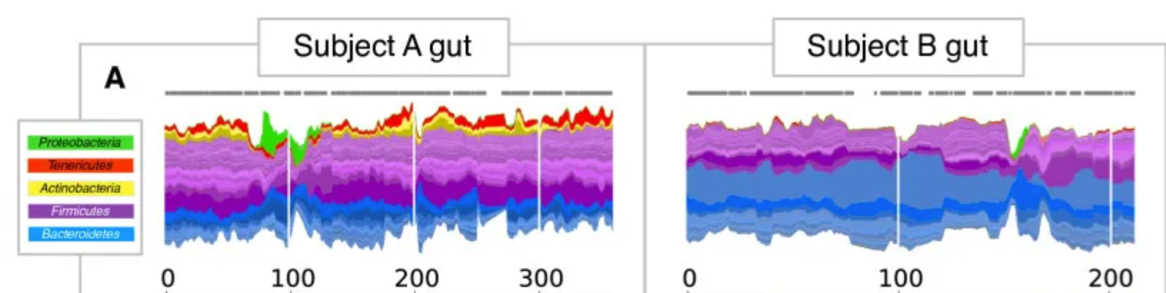
\includegraphics[scale=0.6]{Picture1.png}
 \end{center}
 \caption{一年間にわたる2人(Subject A、Subject B)の糞便を採集したデータ\cite{pmid25146375}\newline
横軸は時点を表す.各ストリームはOTUを表し,ストリーム幅は特定の時点での相対的なOTUの存在量を表す.OTUは,微生物学において種を区別するための操作的分類単位であり,一般にrDNAおよび類似率閾値を使用して分類される.}\label{fig:1.1}
\end{figure}

\section{研究目的}

先行研究では,ヒト腸内細菌叢データについて単純な時系列解析を行い,ホストのライフスタイルとの関連性を解釈した.しかし,ヒト腸内細菌叢の状態の変遷は健康にどのような影響を与えるのかは解析されていない.そこで,本研究では隠れマルコフモデルを用いてヒト腸内細菌叢データを解析することにより,健康との関連性を見出すことを目的とする.




\chapter{手法}

本研究では,観測変数が多項分布に従っている隠れマルコフモデル(HMM)を使う.パラメータの最尤推定における更新式を導出してから,ヒト腸内細菌叢データを導入して解析する.

\section{隠れマルコフモデル}

隠れマルコフモデル(Hidden Markov Model;HMM)は,マルコフ過程をとる隠れ状態に対応する観測状態としてデータを扱う生成確率モデルである\cite{元田_栗田_樋口_松本_村田201202}.
\begin{figure}[h]
\centering
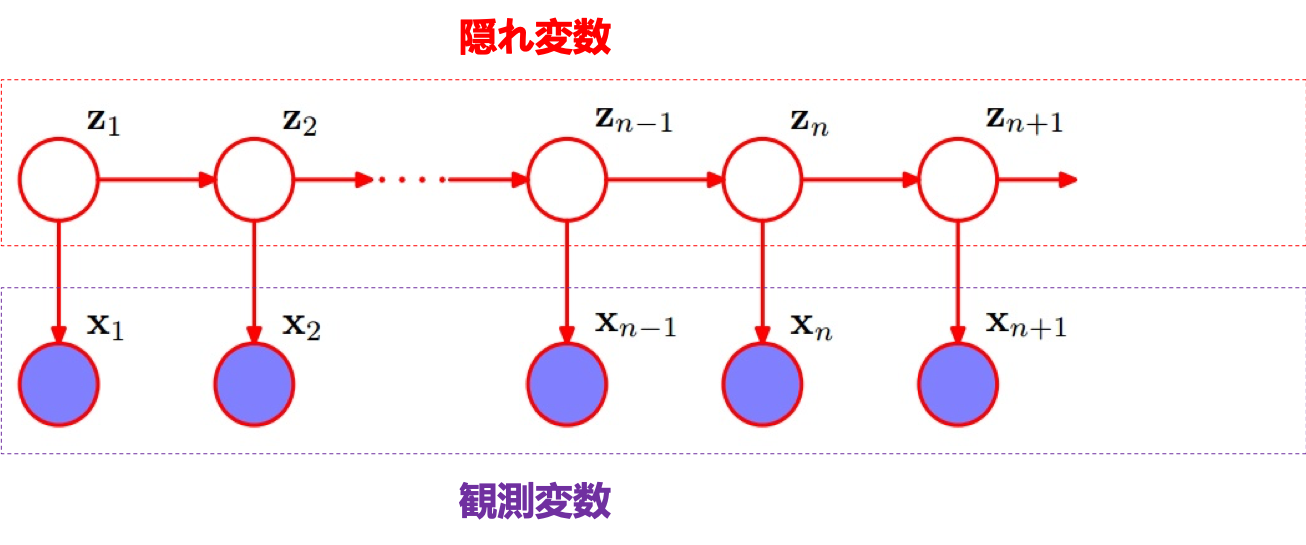
\includegraphics[scale=0.5]{Picture2.png}
\caption{\label{fig:2.1}
隠れマルコフモデル(HMM)のグラフィカル表現\cite{Bishop201002}\newlineここで,観測変数系列$X:=\{\bm{x}_n,n=1,\dots,N\}$は実際に観測・取得することが出来るデータであり,潜在変数系列$Z:=\{\bm{z}_n,n=1,\dots,N\}$は実際に観測・取得する事が出来ないデータである.ここで,潜在変数系列は必ず離散分布に従っている.}
\end{figure}
観測変数$\bm{x}_n$は潜在変数$\bm{z}_n$に影響を受けて生成され,潜在変数$\bm{z}_n$は一次マルコフ連鎖に従い$\bm{z}_{n-1}$の影響を受けて生成される.この条件を満たすように構築したモデルの一つが隠れマルコフモデルであり,潜在変数系列$Z$と観測変数系列$X$の同時確率分布を
\begin{align*}
	p(X,Z) = p(\bm{x}_1,\dots,\bm{x}_N,\bm{z}_1,\dots,\bm{z}_N) &:= p(\bm{z}_1) \left[ \prod_{k=2}^N p(\bm{z}_k|\bm{z}_{k-1})\right] \prod_{k=1}^N p(\bm{x}_k|\bm{z}_k)
	\label{eq:HMM}
\end{align*}
と表すことができる.
潜在変数系列$Z$については,各時点$n$での状態を表す潜在変数$\bm{z}_n,n \in \{1,\dots,N\}$を$K$次元ベクトル空間$\mathbb{K}$上の元とすると,
\begin{align}
    \begin{aligned}
    	\bm{z}_n &= 
	    \begin{pmatrix}
		    z_{n1} \\
		    z_{n2} \\
		    \vdots \\
		    z_{nK}
	    \end{pmatrix} \\
        z_{nk} &\in \{ 0,1 \}, ^\forall n \in \{1,\dots,N\}, ^\forall k \in \{1,\dots,K\} \\
	    & \sum_{k=1}^{K} z_{nk} = 1, ^\forall n \in \{1,\dots,N\}
    \end{aligned}
\end{align}
と書くことができる。さらに,潜在状態間の遷移を表す条件付き分布$p(\bm{z}_n|\bm{z}_{n-1})$を特徴づけるパラメータ,$K \times K$行列$A$を導入する.
この行列$A$の各成分は
\begin{align}
    A_{jk} := p(z_{nk}=1|z_{n-1,j}=1)
	\label{}
\end{align}
として定義するものであり,解釈としては潜在変数の状態が状態$j$から状態$k$へと遷移する確率である.遷移確率であることから行列$A$は規格化されており,
\begin{align}
	\sum_{k=1}^{K} A_{jk} = 1 , ^\forall j \in \{1,2,\dots,K \}
	\label{}
\end{align}
が成立する.$z_{nk} \in \{0,1\} ,^\forall n \in \{1,\dots,N\},^\forall k \in \{1,\dots,K\}$であることから,遷移確率の条件付き分布$p(\bm{z}_n|\bm{z}_{n-1})$は
\begin{align}
    p(\bm{z}_n|\bm{z}_{n-1}) := p(\bm{z}_n|\bm{z}_{n-1},A) = \prod_{k=1}^K \prod_{j=1}^K (A_{jk})^{z_{n-1,j} \times z_{nk}}
    \label{ref:def_A}
\end{align}
と書くことができる.

潜在変数の初期状態$\bm{z}_1$も同様に$K$次元ベクトルのパラメータ$\bm{\pi}\in \mathbb{K}$を
\begin{align}
    \begin{aligned}
        \bm{\pi} &=
        \begin{pmatrix}
            \pi_1 \\
            \pi_2 \\
            \vdots \\
            \pi_{K}
        \end{pmatrix} \\
        \sum_{k=1}^K \pi_k &= 1
    \end{aligned}
    \label{}
\end{align}
と導入することで特徴づけてやることにより
\begin{align}
    p(\bm{z}_1) := p(\bm{z}_1|\bm{\pi}) = \prod_{k=1}^K \pi_k^{z_{1k}}
    \label{}
\end{align}
とすることができる.

最後に,出力確率については,潜在変数$\bm{z}$に依存して変化する分布を特徴づけるパラメータベクトル$\bm{\phi}$を
\begin{align}
    \bm{\phi}= 
    \begin{pmatrix}
        \phi_1 \\
        \phi_2 \\
        \vdots \\
        \phi_K
    \end{pmatrix}
    \label{}
\end{align}
とおくと,
\begin{align}
    p(\bm{x}_n|\bm{z}_n) := p(\bm{x}_n|\bm{z}_n,\bm{\phi}) = \prod_{k=1}^{K} p(\bm{x}_n|\phi_k)^{z_{nk}}
\end{align}
と書くことができる.

以上で導入したパラメータ$A,\bm{\pi},\bm{\phi}$をまとめて$\theta := \{\bm{\pi},A,\bm{\phi}\}$と書く.これを使って隠れマルコフモデルの式を改めて書きなおすと
\begin{align}
	p(X,Z|\theta)=p(\bm{x}_1,\dots,\bm{x}_N,\bm{z}_1,\dots,\bm{z}_N|\theta) = p(\bm{z}_1|\bm{\pi}) \left[ \prod_{k=2}^N p(\bm{z}_k|\bm{z}_{k-1},A)\right] \prod_{k=1}^N p(\bm{x}_k|\bm{z}_k,\bm{\phi})
	\label{eq:def_HMM}
\end{align}
とすることができる.

\section{HMMの最尤推定}

データ集合$\bm{X}=\{\bm{x}_1,\cdots,\bm{x}_N\}$が観測された場合,HMMのパラメータ$\theta := \{\bm{\pi},A,\bm{\phi}\}$を最尤推定によって求めることができる.
まず観測変数系列$X$と潜在変数系列$Z$の同時分布関数$p(X,Z|\theta)$を$Z$について和を取ることで周辺化し,
尤度関数を導入する.すなわち,
\begin{align}
	p(X|\theta) = \sum_{Z} p(X,Z|\theta)
	\label{}
\end{align}
となる.この尤度関数$L(\theta|X)$を直に最大化し最尤推定を実行しようとすると$\sum_Z$の計算をする事になるが,$N$個ある潜在変数系列に対して各々$K$個の状態を取るので結局$K^N$項の和を計算する事になるので,データサイズが大きければ実質不可能となる.
ここではこの困難を克服するためにEMアルゴリズムを用いる.
EMアルゴリズムは2つのステップ
\begin{itemize}
    \item Eステップ:現在推定されている潜在変数の分布に基づいて,モデルの尤度の期待値を計算
    \item Mステップ:Eステップで求まった尤度の期待値を最大化するパラメータを求める
    
\end{itemize}
で構成されているアルゴリズムであり,それぞれ交互に繰り返すことによりパラメータを推計するアルゴリズムである.

\subsection{Eステップ}

Eステップでは,最初にパラメータをある適当な値$\theta^{old}$と設定し,潜在変数の事後分布$p(Z|X,\theta^{old})$を求め,完全データに対する尤度関数の対数の期待値$Q(\theta,\theta^{old})$を
\begin{align}
    \begin{aligned}
	    Q(\theta,\theta^{old}) &= \sum_{Z} p(Z|X,\theta^{old}) \ln p(X,Z|\theta)
    \end{aligned}
    \label{eq:def_Q}
\end{align}
として求める.

ここで,潜在変数$\bm{z}_n$の周辺事後分布$\gamma(\bm{z}_n)$、2つの連続した潜在変数に対する同時分布$\xi(\bm{z}_{n-1},\bm{z}_n)$を
\begin{align} 
    \gamma(\bm{z}_n)           &:= p(\bm{z}_n|X,\theta^{old}) ,        & \gamma:\mathbb{K} \to [0,1] \\
    \xi(\bm{z}_{n-1},\bm{z}_n) &:= p(\bm{z}_{n-1},\bm{z}_n|X,\theta^{old}), & \xi:\mathbb{K}\times\mathbb{K} \to [0,1]
	\label{}
\end{align}
とおく.これに従い,$\gamma(\bm{z}_n),\xi(\bm{z}_{n-1},\bm{z}_n)$について,各要素で
\begin{align}
    \begin{aligned}
        \gamma(z_{nk})           &:= \mathbb{E} \left[ z_{nk} \right]         
            = \sum_{\bm{z}_n} \gamma(\bm{z}_n) z_{nk} = p(z_{nk}=1|X,\theta^{old}) \\
        \xi(z_{n-1,j},z_{nk})    &:= \mathbb{E}\left[ z_{n-1,j} \times z_{nk} \right] 
            = \sum_{\bm{z}_{n-1},\bm{z}_n} \xi(\bm{z}_{n-1},\bm{z}_n)z_{n-1,j}\times z_{nk} = p(z_{n-1,j}=1,z_{nk}=1|X,\theta^{old})
    \end{aligned}
    \label{eq:def_gamma_xi_nk}
\end{align}
とおく.

\eqref{eq:def_HMM}式を\eqref{eq:def_Q}式に代入し、$\gamma,\xi$の定義\eqref{eq:def_gamma_xi_nk}式を用いて変形してくと,$Q(\theta,\theta^{old})$は
\begin{align}
\begin{aligned}
	Q(\theta,\theta^{old}) 
	&= \sum_{Z} p(Z|X,\theta^{old}) \ln p(X,Z|\theta)\\
	&= \sum_{k=1}^{K} \gamma(z_{1k}) \ln \pi_k
   	+  \sum_{n=2}^{N} \sum_{j=1}^{K} \sum_{k=1}^{K} \xi(z_{n-1,j},z_{nk}) \ln A_{jk} 
	+  \sum_{n=1}^{N} \sum_{k=1}^{K} \gamma(z_{nk}) \ln p(\bm{x}_k|\phi_k)
\end{aligned}
	\label{eq:calc_Q}
\end{align}
と変形することができる.

\subsection{Mステップ}

Mステップでは,パラメータ$\theta$を適当に選択することで$Q(\theta,\theta^{old})$の最大化を行う.ここで遷移行列$A$と初期分布$\bm{\pi}$には条件
\begin{align}
    \begin{aligned}
        & \sum_{k}A_{jk} = 1, ^\forall j \in \{1,\dots,K\} \\
        & \sum_{k=1}^{K} \pi_k = 1
    \end{aligned}
\end{align}
が付いてあるため,ラグランジュの未定乗数$(\lambda_1,\dots,\lambda_{K+1})$を導入し,$Q(\theta,\theta^{old})$の最大化問題を解く.数式として
\begin{align}
	\begin{aligned}
        \theta_{max}    &=  \argmax_{\theta=(\bm{\pi},A,\bm{\phi})} F(\bm{\pi}, A, \bm{\phi}) \\ 
        F(\bm{\pi}, A, \bm{\phi}) &:= Q(\theta, \theta^{old}) - \lambda_1\left(\sum_{k=1}^{K} \pi_k - 1 \right) - \sum_{j=1}^{K} \lambda_{j+1} \left( \sum_{k=1}^{K} A_{jk} - 1 \right)\\ 
	\end{aligned}
\label{}
\end{align}
と表され,$F(\pi, A, \phi)$を$\pi,A$の各ベクトル・行列要素で微分することで
\begin{align}
	\begin{aligned}
		\frac{\partial F}{\partial \pi_k}  &= \frac{\gamma(z_{1k})}{\pi_k} - \lambda_1 = 0, 
			\pi_k = \frac{\gamma(z_{1k})}{\lambda_1}  \\
		\frac{\partial F}{\partial A_{jk}} &= \frac{\sum_{n=2}^{N} \xi(z_{n-1,j},z_{nk})}{A_{jk}} - \lambda_{j+1}, 
			A_{jk} = \frac{\sum_{n=2}^{N} \xi(z_{n-1,j},z_{nk})}{\lambda_{j+1}} 
	\end{aligned}
	\label{eq:lagrange_pi_A}
\end{align}
とすることができる.パラメータ$\bm{\phi}$についての微分は観測変数$x$がどのような分布に従うと設定するかに応じて結果が変わるものであるため,次のセクションに示すことにする.\eqref{eq:lagrange_pi_A}を拘束条件であるに代入すると
\begin{align}
	\begin{aligned}
		\sum_{k=1}^{K} \pi_k  &=  \sum_{k=1}^{K} \frac{\gamma(z_{1k})}{\lambda_1}  = 1,
			\therefore \lambda_1 = \sum_{j=1}^{K} \gamma(\bm{z}_{1j}) \\
		\sum_{k=1}^{K} A_{jk} &=  \sum_{k=1}^{K} \frac{\sum_{n=2}^{N} \xi(z_{n-1,j},z_{nk})}{\lambda_{j+1}} =1,
        \therefore \lambda_{j+1} = \sum_{l=1}^{K} \sum_{n=2}^{N} \xi(z_{n-1,j},z_{nl})
	\end{aligned}
	\label{eq:lagrange_lambda}
\end{align}
と求められる.式\eqref{eq:lagrange_lambda}の結果を式\eqref{eq:lagrange_pi_A}に代入すると
\begin{align}
	\begin{aligned}
		\pi_k &=  \frac{\gamma(z_{1k})}{\lambda_1} = \frac{\gamma(z_{1k})}{\sum_{j=1}^{K} \gamma(\bm{z}_{1j})} \\
        A_{jk} &= \frac{\sum_{n=2}^{N} \xi(z_{n-1,j},z_{nk})}{\lambda_{j+1}} =  \frac{\sum_{n=2}^{N} \xi(z_{n-1,j},z_{nk})}{ \sum_{l=1}^{K} \sum_{n=2}^{N} \xi(z_{n-1,j},z_{nl})}
	\end{aligned}
	\label{eq:update_param}
\end{align}
と求められる.

\section{HMMの更新式}

本研究で用いているヒト腸内細菌叢の時系列データは,1年間にわたる32種類のPhylumの存在量であり,多項分布に従うと見なすことができる.そこで,HMMにおいてパラメータ$\bm{\phi}$および出力確率の更新式を導出する必要があると考えられる.これに伴い,EMアルゴリズムにおけるパラメータ$\bm{\phi}$の数式を導出することになる.

まず,パラメータ$\bm{\phi}$の平均を$\bm{\mu}$とすると,観測変数の分布は
\begin{align}
    p(\bm{x}_n|\bm{\phi}_k) &= \frac{M!}{x_{n1}! \dots x_{nD}!} \prod_{i=1}^{D} \bm{\mu}_{ik}^{x_{ni}}
\end{align}
と書くことができる.ここで、Mは試行回数を表す。これを式\eqref{eq:calc_Q}に代入すると
\begin{align}
    Q(\theta,\theta^{old})&= \sum_{k=1}^{K} \gamma(z_{1k}) \ln \pi_k
   	+  \sum_{n=2}^{N} \sum_{j=1}^{K} \sum_{k=1}^{K} \xi(z_{n-1,j},z_{nk}) \ln A_{jk} 
	+  \sum_{n=1}^{N} \sum_{k=1}^{K} \gamma(z_{nk}) \sum_{i=1}^{D} x_{ni} \ln {\mu}_{ik}^{x_{ni}}
\end{align}
と書くことができる.

ここで、$\bm{\mu}_{ik}$は制約条件$\sum_{i=1}^{D}\mu_{ik}=1$を持つため、ラグランジュの未定乗数を用いてラグランジアンは
\begin{align}
    L &= Q(\theta, \theta^{old}) + \lambda_1(\sum_{i=1}^{D} \mu_{i1} - 1) + \dots + \lambda_{k} ( \sum_{i=1}^{D} \mu_{ik} - 1 )
\end{align}
とおく.この関数Lを$\bm{\mu}_{ik}$で微分すると、停留条件により0
\begin{align}
    \frac{\partial L}{\partial \mu_{ik}} &= \frac{\sum_{n=1}^{N} \gamma(z_{nk}) x_{ni}}{\mu_{ik}} + \lambda_{k} = 0 \\
    \mu_{ik} &= \frac{\sum_{n=1}^{N} \gamma(z_{nk}) x_{ni}}{-\lambda_{k}}
\end{align}
となる.$\bm{\mu}_{ik}$の制約条件により
\begin{align}
    \sum_{i=1}^{D} \mu_{ik}&= \sum_{i=1}^{D} \frac{\sum_{n=1}^{N} \gamma(z_{nk}) x_{ni}}{-\lambda_{k}} = 1 \\
    \lambda_{k} &= \sum_{i=1}^{D} \sum_{n=1}^{N} \gamma(z_{nk}) x_{ni} = \sum_{n=1}^{N} \gamma(z_{nk})
\end{align}
となるため,$\bm{\mu}_{ik}$は
\begin{align}
    \mu_{ik} &= \frac{\sum_{n=1}^{N} \gamma(z_{nk}) x_{ni}}{\sum_{n=1}^{N} \gamma(z_{nk})}
\end{align}
と書くことができる.

\chapter{まとめ}

\chapter*{謝辞}
本研究を進めるにあたり,研究の相談,指導をして下さった浜田道昭教授にお礼申し上げます.また研究に関して様々な助言・指導をして下さった細田至温,宮原雅人,白鳥哲嗣様に感謝を申し上げます.さらに日頃より研究に対して議論して下さった浜田研究室の方々にも感謝申し上げます.



\bibliographystyle{unsrt}
\bibliography{ref}

\clearpage

\appendix 

\chapter{補遺}








\end{document}